% Source for accuracy.pdf (sample figure). Build: xelatex accuracy.tex
\documentclass[border=2pt]{standalone}
\usepackage{fontspec}
\setmainfont{TeX Gyre Termes}
\usepackage{unicode-math}
\setmathfont{TeX Gyre Termes Math}
\usepackage{pgfplots}
\pgfplotsset{compat=1.18}
\begin{document}
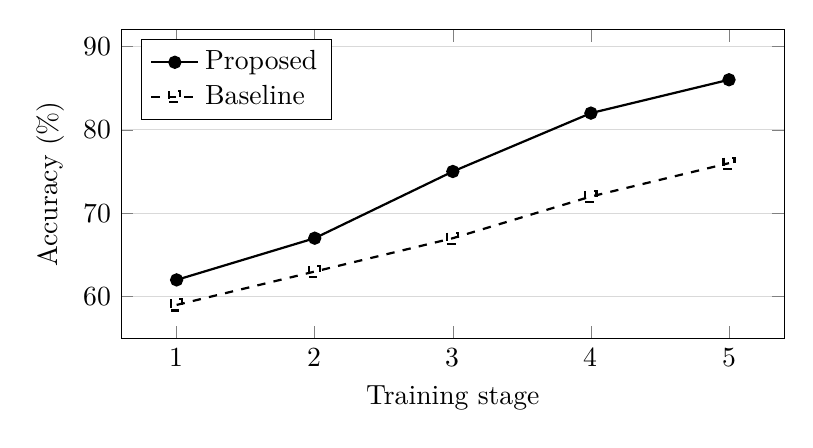
\begin{tikzpicture}
\begin{axis}[width=10cm,height=5.5cm,xlabel={Training stage},
  ylabel={Accuracy (\%)},xtick={1,...,5},ymin=55,ymax=92,
  ymajorgrids,grid style={gray!30},legend pos=north west,
  legend cell align=left]
\addplot[mark=*,thick] coordinates {(1,62)(2,67)(3,75)(4,82)(5,86)};
\addplot[mark=square,thick,dashed] coordinates {(1,59)(2,63)(3,67)(4,72)(5,76)};
\legend{Proposed,Baseline}
\end{axis}
\end{tikzpicture}
\end{document}
